\begin{figure}[h!]
    \begin{center}
    \caption{Effects on Fertility and Birth Outcomes}\label{fig:18}
    \begin{subfigure}{0.32\textwidth}
        \caption{\scriptsize Rates of Birth per Woman (10-49y)}\label{fig:18a}
        \centering
        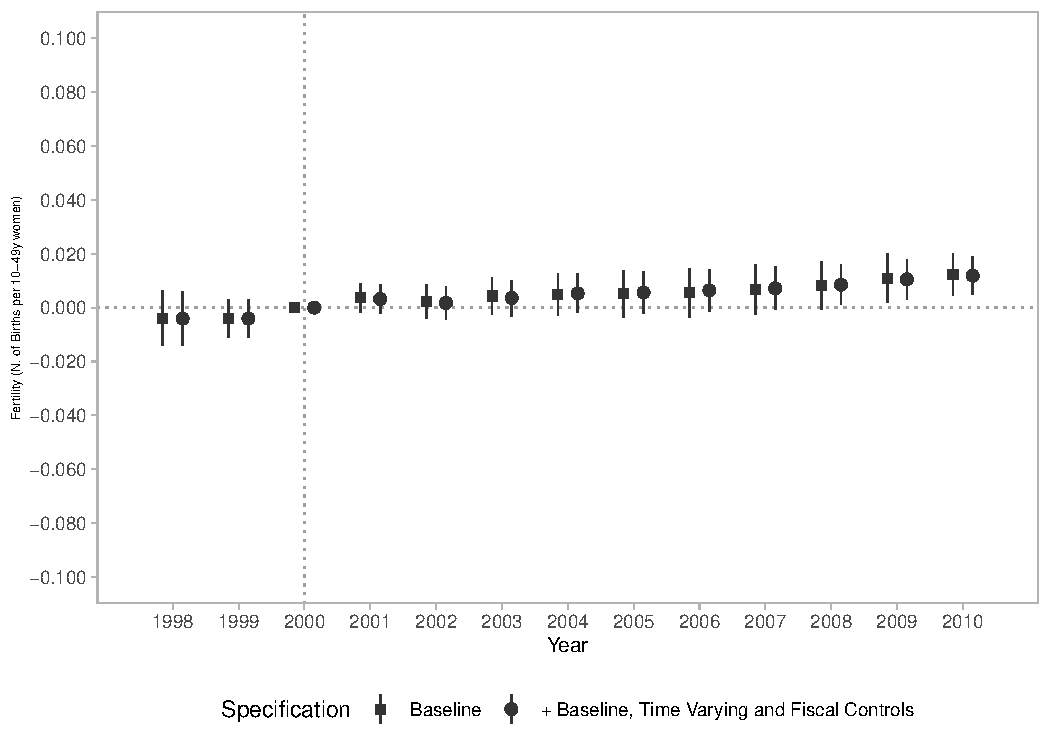
\includegraphics[width=\textwidth]{plots/birth_fertility_dist_ec29_baseline_dist_ec29_baseline_18.pdf}
    \end{subfigure}
    \begin{subfigure}{0.32\textwidth}
        \centering
        \caption{\scriptsize Apgar 1}\label{fig:18b}
        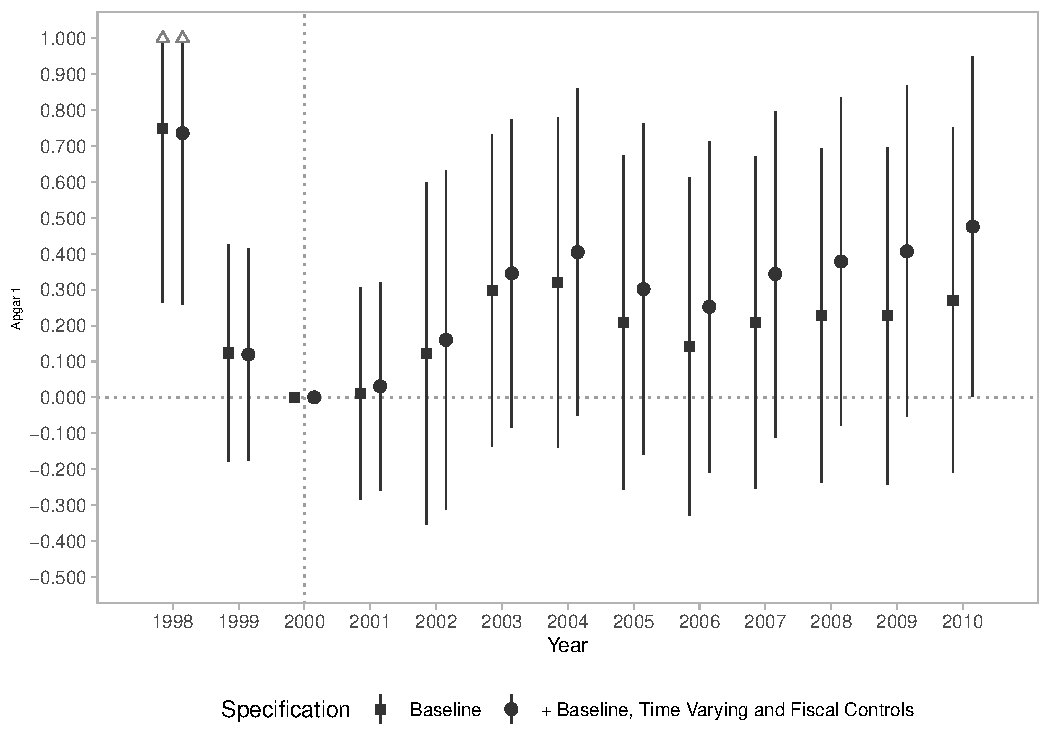
\includegraphics[width=\textwidth]{plots/birth_apgar1_dist_ec29_baseline_dist_ec29_baseline_18.pdf}
    \end{subfigure}
    \begin{subfigure}{0.32\textwidth}
        \centering
        \caption{\scriptsize Apgar 5}\label{fig:18c}
        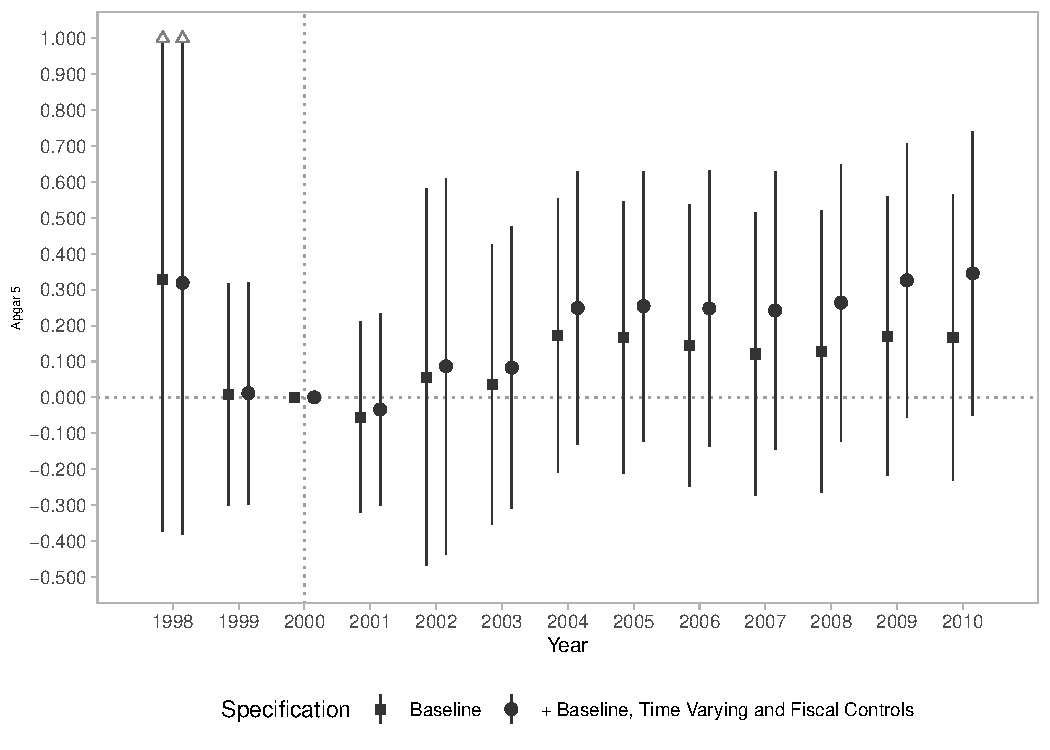
\includegraphics[width=\textwidth]{plots/birth_apgar5_dist_ec29_baseline_dist_ec29_baseline_18.pdf}
    \end{subfigure}
    \begin{subfigure}{0.32\textwidth}
        \caption{\scriptsize Low Birth Weight (<2.5k)}\label{fig:18d}
        \centering
        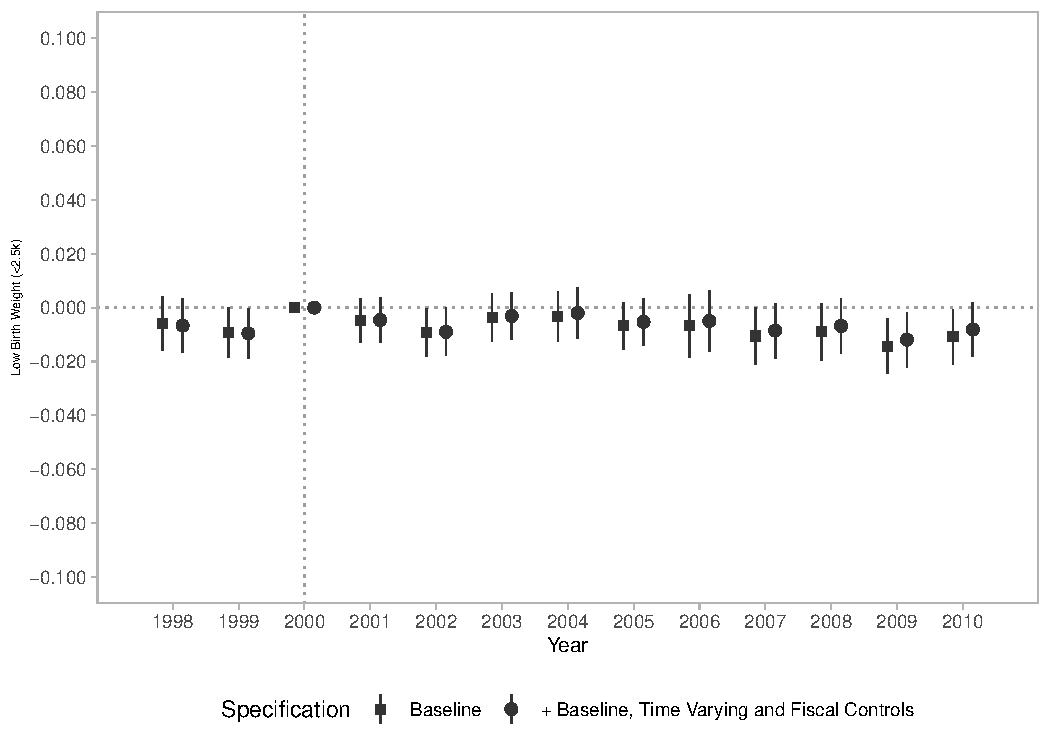
\includegraphics[width=\textwidth]{plots/birth_low_weight_2500g_dist_ec29_baseline_dist_ec29_baseline_18.pdf}
    \end{subfigure}
    \begin{subfigure}{0.32\textwidth}
        \centering
        \caption{\scriptsize Premature Birth}\label{fig:18e}
        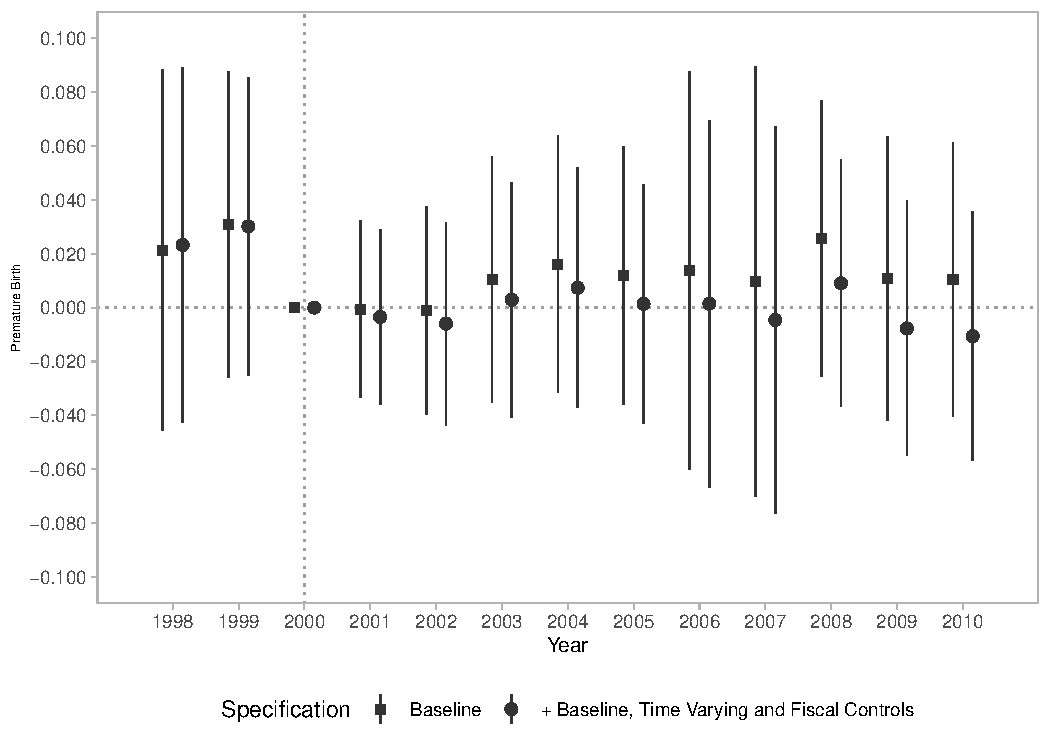
\includegraphics[width=\textwidth]{plots/birth_premature_dist_ec29_baseline_dist_ec29_baseline_18.pdf}
    \end{subfigure}
    \begin{subfigure}{0.32\textwidth}
        \centering
        \caption{\scriptsize Sex Ratio at Birth}\label{fig:18f}
        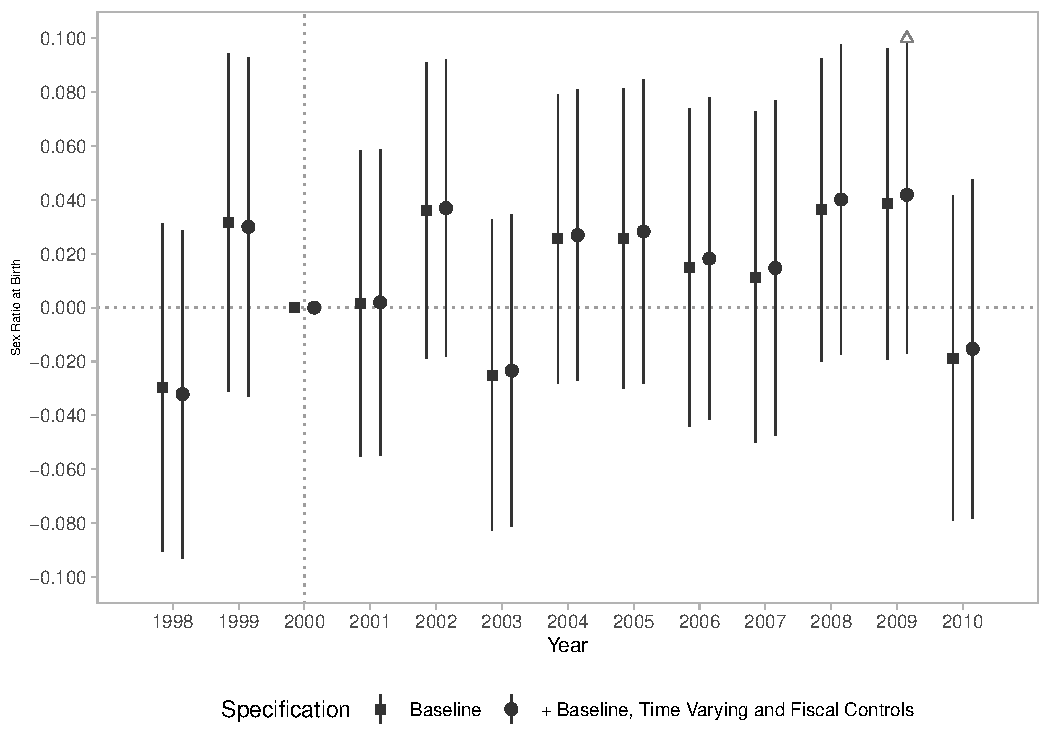
\includegraphics[width=\textwidth]{plots/birth_sexratio_dist_ec29_baseline_dist_ec29_baseline_18.pdf}
    \end{subfigure}
    
    \end{center}
    
            \scriptsize{Notes: The number of observations is 64482 for \ref{fig:18a}, 63705 for \ref{fig:18b}, 59524 for \ref{fig:18c}, 64481 for \ref{fig:18d} and \ref{fig:18e}, and 64470 for \ref{fig:18f}. DiD Estimates from Equation \ref{eq:2}. Independent variable is the distance to the EC/29 target in p.p. Square dots represent the baseline model with municipality and state-year fixed effects. Round dots represent fully saturated specification (Column 4 in regression Tables). Lines represent 95\% confidence intervals. Arrows, when present, indicate confidence intervals out of the plot bounds. Standard errors are clustered in the municipality level.}
    
\end{figure}